\chapter{黑白图像着色}
\label{cha:3-image-color}

  基于wGAN的架构,我们训练了几种模型用于黑白图像着色,下面介绍我们的网络结构以及相关训练参数。

\section{判别器网络}
\label{sec:3-d-net}
  
  判别器网络我们使用了比较常见的CNN网络,其详细参数如下:对于分辨率为64x64的图像,判别器中有4层卷积层与其对应的BN层和LeakyReLU层,每个卷积核均为4,步幅为2,边缘填充为1。这样每个卷积层都是图像分辨率减半,特征通道数翻倍。在得到4x4的特征后,再经过一个卷积核为4,步幅为1,边缘填充为0的卷积层,就得到输出的1x1的结果,即判别器给出的图像是真实的概率。
  
\section{生成器网络}
\label{sec:3-g-net}

  生成器网络是GAN中最重要的一部分,因为它的是否合适决定了最终生成器能否生成理想的结果。我们尝试了基线模型,变分自编码器与U-NET几种结构。对于着色问题而言,我们在所有的生成器网络结构中都没有使用池化层,因为池化层是通过压缩空间上的信息来降低分辨率,这样会丢失一些信息,所以我们都是通过步幅大于1的卷积层达到压缩的目的。

\subsection{基线模型}
\label{sec:3-fcn}
  
  着色问题与一般分类、回归问题的很大不同在于,着色的输入输出分辨率是一样的,在网络中传递时空间上的信息需要得到很好的保持。于是我们最初尝试了一个最简单的网络结构:五个卷积层及其对应的BN层和ReLU层,其中前三个卷积层均核为3,步幅为1,以及1的边缘填充。这样在前三层图像的分辨率都没有变化。后两层卷积层核为1,步幅为1,边缘填充为0,这样在后两层图像分辨率也不发生变化。最后一层卷积层不带BN层与ReLU层。网络结构如图~\ref{fig:fcn}所示。

  \begin{figure}[H]
    \centering
    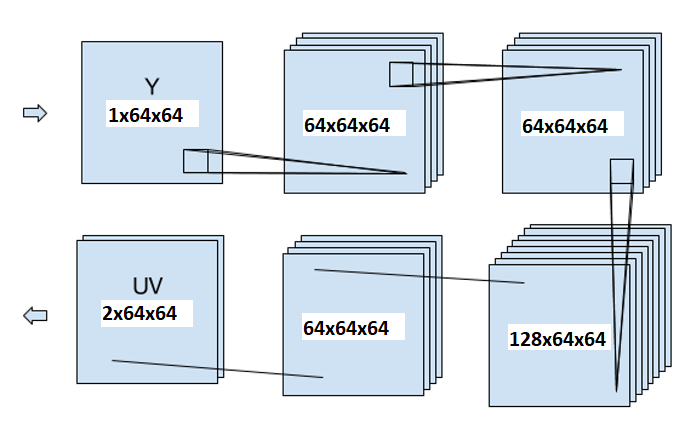
\includegraphics{fcn}
    \caption{基线模型}
    \label{fig:fcn}
  \end{figure}

  另外一个选择是是网络层的通道数,输入的灰度图像通道为1,输出的色度图像通道为2,中间的卷积层通道数为64或128,翻倍以后再减半回来。通道数的数量在一定程度上代表了网络的最大学习能力,所以在网络使用了较多的特征通道。

\subsection{变分自编码器}
\label{sec:3-vae}

  变分自编码器的结构在相关工作中已经介绍过了,在我们的网络中做了一些简化,结构如图~\ref{fig:vae-2},称为编码解码模型(encoder-and-decoder)。

  \begin{figure}[H]
    \centering
    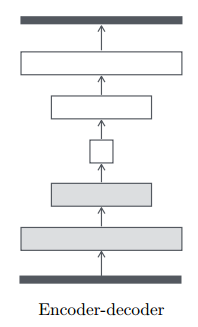
\includegraphics{vae_2}
    \caption{编码解码模型结构示意}
    \label{fig:vae-2}
  \end{figure}

  该模型与基线模型的一点区别在于,网络卷积中图像分辨率是变化的,是一个先缩小后变大还原,即卷积与反卷积的过程,卷积的部分就是编码器,反卷积的部分就是解码器。编码器会将图像压缩到分辨率为1x1的特征向量,然后解码器将这个特征向量(即GAN模型中的随机变量)映射到色度图像。

  这个模型的详细参数如下:对于分辨率为64x64的图像,编码器包含6层卷积层及其对应的BN层和ReLU层,每个卷积层均核为4,步幅为2,边缘填充为1。每个步幅为2的卷积层都会让图像在空间上减半,特征通道上翻倍(有几个卷积层保持而不翻倍通道数)。这样图像经过编码器后得到1x1x256的特征向量。解码器包含6个反卷积层及其对应的BN层和ReLU层,每个反卷积层均核为4,步幅为2,边缘填充为1。每个步幅为2的反卷积层都会让图像在空间上翻倍,特征通道上减半(与编码器网络对应)。这样解码器输出双通道原始分辨率的图像,最后再经过一个tanh的激活函数,这在图像生成的问题上被证明是很有用的。编码器中的ReLU激活函数是LeakyReLU,而解码器中是ReLU。

\subsection{U-NET}
\label{sec:3-unet}

  U-NET的网络结构与编码解码模型非常类似,不过在编码器与解码器的堆成卷积层(即分辨率)之间添加了捷径,即将编码器卷积层得到的特征信息连接到到解码器对应的卷积层一起输入,如图~\ref{fig:unet}所示,这样的好处是编码器中的特征有助于在解码阶段的空间信息恢复。U-NET的结构由Ronneberger~\cite{DBLP:journals/corr/RonnebergerFB15}等人2015提出,被用于生化领域的图像分割。Isola~\cite{DBLP:journals/corr/IsolaZZE16}等人在pix2pix论文中使用了这种结构,他们的任务是不同图像之间的转换,例如猫的手绘轮廓与猫的图片之间的转换,也是图像生成的范围,去掉了会丢失信息的池化层。所以我们的U-NET结构也是学习了他们的模型。

  \begin{figure}[H]
    \centering
    \subcaptionbox{原始U-NET结构\label{fig:unet_origin}}
      {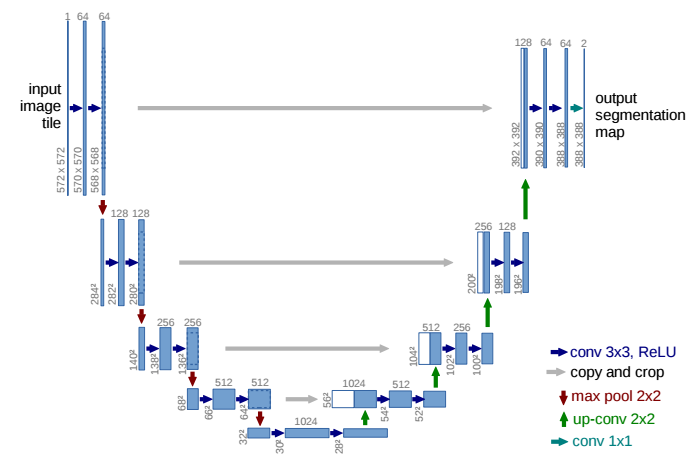
\includegraphics[width=0.45\paperwidth]{unet_origin}}
    \hspace{4em}
    \subcaptionbox{我们的U-NET结构示意\label{fig:unet}}
        {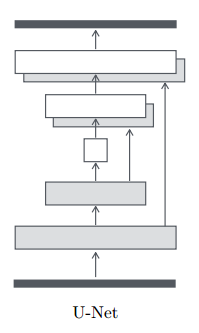
\includegraphics[width=0.15\paperwidth]{unet}}
    \caption{U-NET网络结构}
    \label{fig:unet}
  \end{figure}

\section{训练参数}
\label{sec:3-train}

  训练的相关参数如表~\ref{tab:3-image-train}。

  \begin{table}[h]
    \centering
    \begin{minipage}[t]{0.8\linewidth}
    \caption{黑白图像着色GAN训练参数}
    \label{tab:3-image-train}
      \begin{tabularx}{\linewidth}{lXX}
        \toprule[1.5pt]
        {\heiti 参数名} & {\heiti 描述} & {\heiti 参数值} \\\midrule[1pt]
        image size & 图像分辨率 & 64x64 \\
        batch size & 批处理大小 & 64 \\
        epochs & 重复训练次数 & 200 \\
        ndf & 判别器第一层特征通道数 & 64 \\
        ngf & 生成器第一层特征通道数 & 64 \\
        learn rate D & 判别器学习率 & $5\times10^{-5}$ \\
        learn rate G & 生成器学习率 & $5\times10^{-5}$ \\
        D iterations & 每迭代一次生成器,判别器的迭代次数 & 5 \\
        clamp & 固定判别器参数的常数 & $\pm0.01$ \\
        optimizer & 优化函数 & RMSprop \\
        \bottomrule[1.5pt]
      \end{tabularx}
    \end{minipage}
  \end{table}

  下面对训练参数进行一些解释。图像分辨率使用了较低的64x64,因为图像分辨率增大会使得训练困难以及变慢,所以在初期均使用了较低的分辨率,以达到快速学习,验证模型可行性的目的;D iterations参数的意义是在训练的初期多进行判别器的训练,使得判别器一开始处于一个较准确的状态,从而帮助生成器学习;RMSprop优化函数是深度学习的奠基人之一Geoffrey Hinton~\cite{Tieleman2012}提出的,其目的是解决Adaptive Gradient中学习速率趋向于0的问题。

  另外,我们已经知道生成器的输入是单通道的灰度图像,输出是双通道的色度图像,在这里我们使用的分别是YUV色彩空间的Y通道与UV通道,训练图像的YUV值均归一化到[-1,1]。